\documentclass[12pt]{article}
\usepackage[answers]{finalxm}
\usepackage{pdflscape}	% for landscape layout on specific page 
\usepackage{listings}
\lstset{basicstyle=\ttfamily,breaklines=true}
%
% \usepackage{doc}
% docstrip
%
%\graphicspath{{./fig/}}

%%%%%%%%%%%%%%%%%%%%%%%%
%%% SETUP TITLE PAGE %%%
%%%%%%%%%%%%%%%%%%%%%%%%
\mtefe{Akhir}
\semester{Kedua}
\sidang{2017/2018}
\examMonthYear{by}
\courseCode{\LaTeX101}
\courseNameEn{Manual for Writing Exam Paper Using \LaTeX}
\courseNameBM{x}
\durationhr{1}
\pagesbm{THIRTY ONE}

\renewcommand{\makecover}{
	\pagestyle{titlestyle}
	\vspace*{5\baselineskip}
	\hrule \vspace*{2\baselineskip}
	\begin{center}
		\textbf{UNIVERSITI MALAYSIA PERLIS}\\[\baselineskip]
		\textbf{Manual for Writing Exam Paper Using \LaTeX }\\
		\textbf{[Manual Menulis Kertas Peperiksaan Menggunakan \LaTeX]} \\[2\baselineskip]
		by \\[\baselineskip]
		Mohd Hanafi Mat Som\\ msmhanafi[at]gmail.com\\[2\baselineskip]
		March 6, 2018\\		
		Revisions:~\today, Ver 2.2 \\[2\baselineskip]
		\hrule \vspace*{2\baselineskip}
	\end{center}
	
	Please make sure that this manual has \textbf{\thelastpageSTR~(\thelastpage)} printed pages including this front page before you start reading.%
	
	\translation{%
		Sila pastikan manual ini mengandungi\textbf{\subnumstr~(\thelastpage)}~muka surat yang bercetak termasuk muka hadapan sebelum anda membaca.%
	}\bigskip
}

\begin{document}
% cover page
%\begin{titlepage}	
\makecover	
%\instructionen{
%	This question paper has \textbf{TWO (2)} parts. Answer \textbf{all} questions in \mbox{\textbf{Part A}} and \mbox{\textbf{THREE (3)}} question in \mbox{\textbf{Part B}}. Each question contributes 25 marks.
%}
%\instructionbm{%
%	Kertas soalan ini mengandungi \textbf{DUA (2)} bahagian. Jawab \textbf{semua} soalan di \mbox{\textbf{Bahagian A}} dan \mbox{\textbf{TIGA (3)}} soalan di \mbox{\textbf{Bahagian B}}. Setiap soalan menyumbang 25 markah.%
%}
%\end{titlepage}

\clearpage
\renewcommand*\contentsname{Table of Contents}
\renewcommand{\setmainstyle}{
	\pagestyle{main}
	\vspace*{1mm}
	\setcounter{page}{3}
}
\tableofcontents

\clearpage

%%%%%%%%%%%%%%%%%%%%%%%%%%%%
%%% MAIN BODY START HERE %%%
%%%%%%%%%%%%%%%%%%%%%%%%%%%%
% setting for header style
\setmainstyle

\section{Introduction}
This section provide explanations of the important commands available in the \texttt{finalxm.sty} package with some examples. Put all files in a folder as \LaTeX~will generate a number of files. \bigskip

\subsection{Package Installation}
The simplest installation require no technical knowledge. The \verb|finalxm.sty| can be used inside a folder containing your \verb|finalxm.tex| file. But as you will create a number of files very semester for mid-term \& final examinations, this method seems not quite right. 

\bigskip
Another method is to put your \verb|finalxm.sty| in the custom TEXMF root directories that are in-compliant with the \LaTeX~tree directory system (TDS).

\subsubsection{MiKTeX}
\begin{enumerate}[topsep=0pt, parsep=0pt]
	\item \label{lbl:step1} Create a directory, say \textbf{\textasciitilde/texmf}, which serves as the new TEXMF root directory. For example, \textbf{D:/Dropbox/texmf}.	
	\item Create TDS-compliant subdirectories (ie. \textbf{D:/Dropbox/texmf/tex/latex/}) 
	\item Start MiKTeX Console and open the \textbf{Settings} page.
	\item Click the \textbf{Directories} tab.
	\item Click the Add button and browse to \textbf{~/texmf} created earlier in step \ref{lbl:step1}.
	\item Copy/move \verb|finalxm.sty| file to \textbf{\textasciitilde/texmf/tex/latex/}
\end{enumerate}

\subsubsection{MacTeX and TeX Live}
\begin{enumerate}[topsep=0pt, parsep=0pt]
	\item Create a directory \textbf{\textasciitilde/Library/texmf} in your home directory, if there is not one there already.	
	\item Install the various package files into subdirectories of texmf as follows:
	\begin{enumerate}
		\item All .bst and .bib files into \textbf{texmf/bibtex} (or subdirectories)
		\item All font-related files into \textbf{texmf/fonts} (or subdirectories)
		\item All documentation files into \textbf{texmf/docs}
		\item All other files (.sty, .cls, .tex, etc.) should go into \textbf{texmf/tex}.		
	\end{enumerate}
\end{enumerate}

\subsection{finalxm.sty Package}\label{package}
The \verb|finalxm.sty| uses a number of packages. You need to install these packages to compile your tex file. If you have setup the MikTeX to install the missing package on-the-fly, then you need not to worry. You can also opt to install these packages manually using the MikTeX console. 

\begin{lstlisting}[basicstyle=\footnotesize, frame=single]
\RequirePackage[T1]{fontenc}
\RequirePackage[utf8]{inputenc}
\RequirePackage{mathptmx}	% closest to times new roman
\RequirePackage{latexsym, amsmath, amssymb, textcomp} % typesetting mathematical symbols, formulae and equations.
\RequirePackage{siunitx}	% si unit 
\RequirePackage[a4paper, top=2.54cm, left=2.54cm, right=2.54cm, bottom=3.17cm, footskip=0.6cm]{geometry}
\RequirePackage{fancyhdr}	% header
\RequirePackage{enumitem}	% enumerate questions
\RequirePackage{fmtcount, zref-lastpage} % for page number
\RequirePackage[dvipsnames]{xcolor}	% font color
\RequirePackage{graphicx, caption}	% figure table 
\RequirePackage{float}	% for figure table float
\RequirePackage{booktabs}	% for table
\RequirePackage{tabularx}
\RequirePackage[bookmarksopen=true]{hyperref}
\RequirePackage[capitalize, nameinlink]{cleveref} %reference
\RequirePackage{framed}	
\RequirePackage{xparse}
\end{lstlisting}

\subsubsection{Options}
The \verb|finalxm.sty| has several options, \verb|minutes|, \verb|answers|, \verb|ftquestionnum|, \verb|ftquestionnumx|, \verb|ppkas|, and \verb|ppkb|. 

\begin{framed}
The \verb|minutes| option will show the duration of examination in both hours and minutes. 

\smallskip 
The \verb|answers| option make all answer visible in the \verb|.pdf| output.

\smallskip 
The \verb|ftquestionnum| option make the numbering for Figure and Table to include part/section and question number ie Figure A1.1, Table B1.1 etc.  

\smallskip 
The \verb|ftquestionnumx| option make the numbering for Figure and Table to include question number ie Figure 1.1, Table B1.1 etc.  

\smallskip 
The \verb|ppkas| option is specific to PPK Alam Sekitar style for Figure and Table caption.

\smallskip 
The \verb|ppkb| option is specific to PPK Bioproses style for Figure and Table caption.
\end{framed}

Start the preamble codes as shown below in your \verb|main.tex| file. In this case, the duration of examination will only take argument for \verb|\@durationhr| that indicate total hours to answer the question. This is the standard for all PPK. 

\begin{lstlisting}[basicstyle=\footnotesize, frame=single]
\documentclass[12pt]{article}	
\usepackage{finalxm}	
\end{lstlisting}

\clearpage  
For PPKAS and PPKB, the preamble is declared, 

\begin{lstlisting}[basicstyle=\footnotesize, frame=single]
% For PPKAS
\documentclass[12pt]{article}	
\usepackage[ppkas, ftquestionnumx]{finalxm}	
\end{lstlisting}

\begin{lstlisting}[basicstyle=\footnotesize, frame=single]
% For PPKB
\documentclass[12pt]{article}	
\usepackage[ppkb, ftquestionnumx]{finalxm}	
\end{lstlisting}

\bigskip
If you need minutes, indicate the option for \verb|finalxm.sty| package as shown in the preamble code below. Then, please define \verb|\durationmin| in your \verb|main.tex|, just below the \verb|\@durationhr|. 

\begin{lstlisting}[basicstyle=\footnotesize, frame=single]
% Standard
\documentclass[12pt]{article}	
\usepackage[minutes]{finalxm} 
\end{lstlisting}

\begin{lstlisting}[basicstyle=\footnotesize, frame=single]
% For PPKAS
\documentclass[12pt]{article}	
\usepackage[ppkas, ftquestionnumx, minutes]{finalxm}	
\end{lstlisting}

\begin{lstlisting}[basicstyle=\footnotesize, frame=single]
% For PPKB
\documentclass[12pt]{article}	
\usepackage[ppkb, ftquestionnumx, minutes]{finalxm}	
\end{lstlisting}

You can write the answers to all questions in the documents and have the option of showing the answer by executing the \verb|answers| option of the \verb|finalxm.sty| package. The preamble codes is shown below. Refer to the \ref{answerscheme} Section in page~\pageref{answerscheme} for guideline on writing the answers scheme. The duration of exam will be replaced by \textbf{ANSWER SCHEME}. 

\begin{lstlisting}[basicstyle=\footnotesize, frame=single]
% Standard
\documentclass[12pt]{article}	
\usepackage[answers]{finalxm} 
\end{lstlisting}

\begin{lstlisting}[basicstyle=\footnotesize, frame=single]
% For PPKAS
\documentclass[12pt]{article}	
\usepackage[ppkas, ftquestionnumx, answers]{finalxm}	
\end{lstlisting}

\begin{lstlisting}[basicstyle=\footnotesize, frame=single]
% For PPKB
\documentclass[12pt]{article}	
\usepackage[ppkb, ftquestionnumx, answers]{finalxm}	
\end{lstlisting}

\clearpage 
Next, define the parameter of your exam in the codes below.

\begin{lstlisting}[basicstyle=\footnotesize, frame=single]
%%%%%%%%%%%%%%%%%%%%%%%%
%%% SETUP TITLE PAGE %%%
%%%%%%%%%%%%%%%%%%%%%%%%
\mtefe{Akhir} 			% Akhir, Pertengahan
\semester{Kedua}		% Pertama, Kedua
\sidang{2017/2018}		
\examMonthYear{Jun 2018}
\courseCode{ENT390}
\courseNameEn{Bioinstrumentation 1}
\courseNameBM{Bioinstrumentasi 1}
\pagesbm{TIGA PULUH SATU}		% used if the number of pages exceeds 30
\durationhr{2}		% duration of exam
\makeatletter 
\if@minutes
	\durationmin{30 Minit}	% MUST be enabled using \usepackage[minutes]{finalxm}
\fi 		
\makeatother
\end{lstlisting}

\bigskip
You need to modify \verb|\pagesbm| \textbf{IF ONLY} the total number of pages of your document \textbf{exceeds} 30 pages. 

\section{List of important commands to note.}

\begin{table}[H]
	\begin{tabularx}{\linewidth}{r X}
		\verb|\makecover|: & begin to make the cover page. \\
		
		\verb|\makecoverend|: & close the process of making cover page. \\
		
		\verb|\setmainstyle|: & setup the document style. \\
		
		\verb|\parten|: & declared as \textbf{Part} \\
		
		\verb|\partbm|: & declared as \textbf{Bahagian} \\
		
		\verb|\newparten{text}|: & start new part AND \textbf{reset} the question number ie \textbf{Part A}. \\
		
		\verb|\newpartenx{text}|: & start new part \textbf{without reseting} the question number. \\
		
		\verb|\newpartbm{text}|: & translation of current part. \\
		
		\verb|\newpartbmx{text}|: & PPKAS style. Translation of section without square bracket and no bold. \\
		
		\verb|\figurebm|: & declared as \textbf{Rajah}. \\
		
		\verb|\figurecaption|: & define the caption for \textbf{Figure} in bahasa \\
		
		\verb|\tablecaption|: & define the caption for \textbf{Table} in bahasa \\
		
		\verb|\jadualbf|: & bold label caption \textbf{Jadual 1} \\ 
		
		\verb|\question{opt. text}[label]|: & define question in English and Bahasa with label to refer.\\
		
		\verb|\partQuestion{opt. text}[label]|: & define question in English and Bahasa. Include Part number ie Question A1 with label to refer\\
		
		\verb|\listbeginx|: & start numbering WITHOUT space before the command. Refer to page \pageref{chemical}.\\
		
		\verb|\listbegin|: & start numbering WITH space before the command. Refer to page \pageref{itm:net}. \\
		
		\verb|\listclose|: & close the \verb|\listbegin| and \verb|\listbeginx| commands.\\
		
		\verb|\item|: & start the question with proper numbering within \verb|\listbegin| and \verb|\listbeginx|.\\ 
		
		\verb|\translation{text}|: & format translation in the curly bracket.\\
		
		\verb|\translationbf{text}|: & format translation in \textbf{bold} in the curly bracket.\\
		
		\verb|\qmarks{5}|: & put 5 marks for the current question.\\
		
		\verb|\answer|: & open environment to write your answer in blue color, small font.\\
		
		\verb|\label{label}|: & put label to the current part of the question. \\
		
		\verb|\ref{label}|: & reference to \verb|\label{label}|. Refer to example in page \pageref{chemical}.\\
		
		\verb|\cref{label}|: & reference to Figure or Table  with hyperlink.\\
		
		\verb|\Cref{label}|: & reference to Rajah or Jadual  with hyperlink.\\		 
		
		\verb|\cref*{label}|: & reference to Figure or Table without hyperlink.\\
		
		\verb|\Cref*{label}|: & reference to Rajah or Jadual  without hyperlink.\\		 
	\end{tabularx}
\end{table}

\begin{table}[H]
	\begin{tabularx}{\linewidth}{r X}		
		\verb|\clearpage|: & start new page. Flush all float prior to command. \\
		
		\verb|\newpage|: & start new page. Do not flush the float prior to command.\\
		
		\verb|\smallskip|: & Inserts a small space in vertical mode (between two paragraphs).\\
		
		\verb|\medskip|: & Inserts a medium space in vertical mode (between two paragraphs).\\
		
		\verb|\bigskip|: & Inserts a big space in vertical mode (between two paragraphs).\\
		
		\verb|\vskip value|: & Inserts a vertical space specified by the somevalue ie. 4em. \\
		\verb|\arraystretch{value}|: & adjust the table row spacing. the standard value can be set \verb|\arraystretch{1.2}|.  
	\end{tabularx}
\end{table}

\subsection{$\backslash$question\{\} and $\backslash$partQuestion\{\}}
The command \verb|\question| will generate output:

%\rule[1.5mm]{\linewidth}{0.5mm}
\begin{framed}
	\textbf{Question 1\\
		\translation{Soalan 1}}
\end{framed}

%\rule{\linewidth}{0.5mm}
%\medskip

Each time you call the \verb|\question| command, the question numbering is being increased by 1. For example, \bigskip

\verb|\question|

\verb|\question|

\verb|\question|\bigskip

will generate output:

\begin{framed}
	\textbf{
		Question 1\\
		\translation{Soalan 1}
	}
	
	\medskip
	\textbf{
		Question 2\\
		\translation{Soalan 2}
	}
	
	\medskip
	\textbf{
		Question 3\\
		\translation{Soalan 3}
	}
	
\end{framed}

If you want the question is numbered such as \textbf{QUESTION A1} based on the parts of the question, you need to declare parts by calling the \verb|\newparten| command. \verb|\newpartbm| is used for the translation of \verb|\newparten| command. The command: \clearpage 

\begin{lstlisting}[basicstyle=\footnotesize, frame=single]
\newparten{Answer all questions} \\
\newpartbm{Jawab semua soalan}

\partQuestion

\partQuestion

\newparten{Answer any THREE (3) questions} \\
\newpartbm{Jawab mana-mana TIGA (3) soalan}

\partQuestion

\partQuestion

\end{lstlisting}

will generate: 

\begin{framed}
	\newparten{Answer all questions} 
	
	\newpartbm{Jawab semua soalan}
	\medskip
	
	\partQuestion{}
	
	\partQuestion{}
	
	\newparten{Answer any THREE (3) questions} 
	
	\newpartbm{Jawab mana-mana TIGA (3) soalan}
	\medskip
	
	\partQuestion{}
	
	\partQuestion{}
\end{framed}

Note that the \verb|\newparten| command will reset the question numbering. There is a special command to suppress the question number from being reset, \verb|\newpartenx|. Note the difference between previous command. \medskip 

\begin{lstlisting}[basicstyle=\footnotesize, frame=single]
\newparten{Answer all questions} \\
\newpartbm{Jawab semua soalan}

\partQuestion

\partQuestion

\newpartenx{Answer any THREE (3) questions} \\
\newpartbm{Jawab mana-mana TIGA (3) soalan}

\partQuestion

\partQuestion
\end{lstlisting}

\begin{framed}
	\setcounter{counterpart}{0}
	\newparten{Answer all questions} 
	
	\newpartbm{Jawab semua soalan}\\
	
	\partQuestion{}
	
	\partQuestion{}
	
	\newpartenx{Answer any THREE (3) questions} 
	
	\newpartbm{Jawab mana-mana TIGA (3) soalan}\\
	
	\partQuestion{}
	
	\partQuestion{}
	
\end{framed}

\verb|\newparten| command \textbf{MUST} be declared to enable the \verb|\partQuestion| command, otherwise it will cause errors during compilation. 

\subsection{$\backslash$parten, $\backslash$partbm and $\backslash$figurebm}
To change the default setting \textbf{Part} to \textbf{Section}, \verb|\renewcommand| must be called. The same goes for \verb|\figurebm| that has default value of \textbf{Rajah}. For example, 

\begin{lstlisting}[basicstyle=\footnotesize, frame=single]
\renewcommand{\parten}{Section}
\renewcommand{\partbm}{Seksyen}
\renewcommand{\figurebm}{Gambarajah}
\end{lstlisting}

will generate \textbf{Section}, \textbf{Seksyen}, and \textbf{Gambarajah}. 

\subsection{Figure and Table}

The \verb|\figurecaption| and \verb|\tablecaption| are used when the caption for figure and table are required such as for PPKAS and PPKB. 

\begin{lstlisting}[basicstyle=\footnotesize, frame=single]
\begin{figure}[H] % H means, to put figure here after the code
	\centerin
	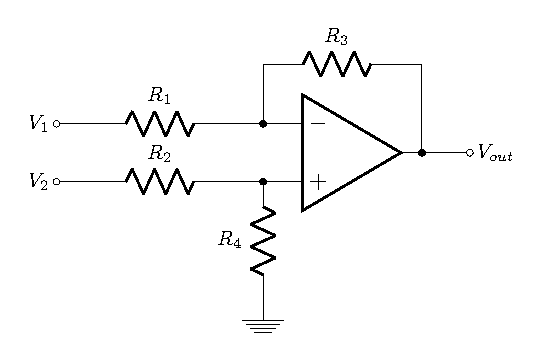
\includegraphics{diffamp}
	\caption{Differential Amplifier \\ \figurecaption{Penguat Pembeza}}
	\label{fig:diffamp}
\end{figure}
\end{lstlisting}

\clearpage
\begin{lstlisting}[basicstyle=\footnotesize, frame=single]
\renewcommand{\arraystretch}{1.2}	% to make better spacing between rows
\begin{table}[H]
\centering
\caption{Frequency vs Magnitude \\ \tablecaption[\jadualbf]{Frekuensi vs Magnitud}}	\begin{tabularx}{220pt}{c c}
	\hline
	\multicolumn{1}{|l|}{\textbf{Frequency}} & \multicolumn{1}{l|}{\textbf{Impedance (Magnitude) ($\Omega$)}} \\
	\hline
		5 Hz  & 20,000 \\
		\vdots     & \vdots \\
		40 kHz & 602 \\
	\hline
\end{tabularx}%
\label{table:freqmag}%
\end{table}%
\end{lstlisting}

You can however mix caption style between standard and PPK specific. The command below must be invoke prior to beginning of figure and table. Then, the next figure/table will follow the new caption style. 

\begin{lstlisting}[basicstyle=\footnotesize, frame=single]
% For PPKAS
\documentclass[12pt]{article}	
\usepackage[ppkas, ftquestionnumx]{finalxm}	

\begin{document}
	%invoke new caption style
	\captionsetup[figure]{labelsep=newline, font=bf} 	
	\begin{figure}[H] % H means, to put figure here after the code
		\centering
		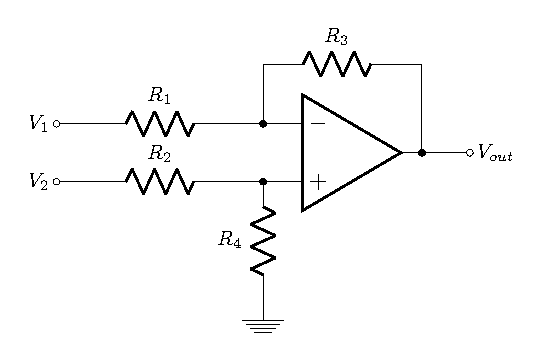
\includegraphics{diffamp}
		\caption{\rajah}
		\label{fig:diffamp}
	\end{figure}
	
	%invoke new caption style
	\captionsetup[table]{labelsep=newline, font=bf} 
	\begin{table}[H]
		\centering
		\caption{\jadual}	
		\begin{tabularx}{220pt}{c c} 
			\hline
			\multicolumn{1}{|l|}{\textbf{Frequency}} & \multicolumn{1}{l|}{\textbf{Impedance (Magnitude) ($\Omega$)}} \\
			\hline
			5 Hz  & 20,000 \\ \vdots & \vdots \\ 40 kHz & 602 \\
			\hline
		\end{tabularx}%
		\label{table:freqmag}%
	\end{table}%
\end{document}
\end{lstlisting}

\clearpage
There are a number of parameters for \verb|\captionsetup|. Important parameters to use for \verb|finalxm.sty| are,

\smallskip
\fbox{font, labelfont, textfont} which can be set to either \texttt{bf, normalfont}. 

\smallskip
\texttt{font} affect all captions, \texttt{labelfont} will only affect ie Figure 1, Table 1. Finally \texttt{textfont} will only affect caption description ie \textit{Differential Amplifier}. 

\smallskip
\fbox{labelsep} which can be set to either \texttt{newline, colon}

\medskip 
\begin{lstlisting}[basicstyle=\footnotesize, frame=single]
\captionsetup[figure]{labelsep=newline, font=bf} 
\captionsetup[figure]{labelsep=colon, labelfont=bf, textfont=normalfont}

\captionsetup[table]{labelsep=newline, font=normalfont} 
\captionsetup[table]{labelsep=colon, labelfont=bf}
\end{lstlisting}
      
\clearpage 
\section{Write Questions in a Single File}

You can make a whole question from a single tex file. It is pretty straight forward. 

\begin{lstlisting}[basicstyle=\footnotesize, frame=single]

%%%%%%%%%%%%%%%%%%%%%%%%%%%%
%%% MAIN BODY START HERE %%%
%%%%%%%%%%%%%%%%%%%%%%%%%%%%
% setting for header style
\setmainstyle

% PART A
\newparten{Answer all questions} \\
\newpartbm{Jawab semua soalan}\\
\bigskip

% QUESTION 1
\question{}[\label{qlabel:chem}]	
\listbeginx	% start 1st level question
	\item \label{chemical} What chemical reactions you expect to see at these electrodes? 
	
	\translation{Apakah tindak balas kimia yang anda jangka dapat dilihat pada kedua-dua elektrod} 
	
	\qmarks{4}	% define marks

	\listbeginx	% start 2nd level question
		\item Based on \ref{chemical}, explain what will happen if the electrodes were shorted together. Explain what will happen if the electrodes were shorted together. 
		
		\translation{Terangkan apakah yang akan berlaku apabila kedua-kedua elektrod disambung?. Terangkan apakah yang akan berlaku apabila kedua-kedua elektrod disambung?} 
		
		\qmarks{2} % define marks
	\listclose % close 2nd level question

	\item Explain what will happen if both electrodes is shorted as described in Q\ref{qlabel:chem}\ref{chemical} 
	
	\translation{Terangkan apakah yang akan berlaku apabila kedua-kedua elektrod disambung?} 	
	
	\qmarks{3} % define marks
\listclose % close 1st level question










% QUESTION 2
\clearpage	% start new page
\question{[CO1,PO1]}

% question without enumerate list
Silver/silver chloride (Ag/AgCl) electrodes are commonly used in biological measurement.\\
\translation{Elektrod Argentum/Argentum chloride (Ag/AgCl) digunakan secara meluas didalam pengukuran biologi}	\\
\qmarks{5}

\listbegin	% start 1st level question
	\item \label{halfmembrane} State the definition of half-membrane \\	
	\translation{Nyatakan definisi separuh-membran}\\	
	\qmarks{2}
	
	\item \label{itm:net} Elaborate the basic mechanisms that contribute to condition in \ref{halfmembrane}, and write its net potential.\\ % use label to reference to the list item	
	\translation{Kembangkan mekanisma asas yang menyumbang kepada keadaan di \ref{halfmembrane}, dan tuliskan upaya bersih.}\\	
	\qmarks{4}		
	
	\listbegin % start 2nd level question
		\item \label{itm:ref2nd} Second level item that refer to \ref{itm:net}. Use 10~\si{\mega\ohm} here. But noted on the use of \si in translation.
		
		\translation{ini adalah level kedua. Gunakan \emph{10~\si{\mega\ohm}} disini. Perhatikan perbezaan penggunaan \si disini dan diatas.} 
	
		\listbeginx % start 3rd level question
			\item Another level. This is third level. This is third level. This is third level. This is third level.
			
			\translation{Ini adalah level ketiga. Ini adalah level ketiga. Ini adalah level ketiga. Ini adalah level ketiga. Ini adalah level ketiga. Ini adalah level ketiga}
		
			\listbeginx  % start 4th level question
				\item Another level. This is fourth level. This is fourth level. This is fourth level. This is fourth level.\\ 				
				\translation{Ini adalah level keempat. Ini adalah level keempat. Ini adalah level keempat. Ini adalah level keempat.}
			\listclose % close 4th level question
		\listclose % close 3rd level question
	\listclose % close 2nd level question
\listclose	% close 1st level question
\paperend
\end{lstlisting}

\clearpage

\setcounter{counterquestion}{0}
\setcounter{counterpart}{0}
% PART A
\newparten{Answer all questions} \\
\newpartbm{Jawab semua soalan}\\

\question{}[\label{qlabel:chem}]
	\listbeginx	% start 1st level question
	\item \label{chemical} What chemical reactions you expect to see at these electrodes? \\
	\translation{Apakah tindak balas kimia yang anda jangka dapat dilihat pada kedua –dua elektrod} \\
	\qmarks{4}	% define marks

	\listbeginx	% start 2nd level question
		\item Based on \ref{chemical}, explain what will happen if the electrodes were shorted together. Explain what will happen if the electrodes were shorted together. \\
		\translation{Terangkan apakah yang akan berlaku apabila kedua – kedua elektrod disambung?. Terangkan apakah yang akan berlaku apabila kedua – kedua elektrod disambung?} \\
		\qmarks{2} % define marks
	\listclose % close 2nd level question
	
	\item Explain what will happen if both electrodes is shorted as described in Q\ref{qlabel:chem}\ref{chemical} \\
	\translation{Terangkan apakah yang akan berlaku apabila kedua – kedua elektrod disambung?} \\
	\qmarks{3} % define marks
\listclose % close 1st level question

\clearpage	% end question and start new page

% QUESTION 2
\question{[CO1,PO1]}

% question without enumerate list
Silver/silver chloride (Ag/AgCl) electrodes are commonly used in biological measurement.\\ 
\translation{Elektrod Argentum/Argentum chloride (Ag/AgCl) digunakan secara meluas didalam pengukuran biologi}	\\
\qmarks{5}

\listbeginx	% start 1st level question
\item \label{halfmembrane} State the definition of half-membrane\\
\translation{Nyatakan definisi separuh-membran}\\
\qmarks{2}
\item \label{itm:net} Elaborate the basic mechanisms that contribute to condition in \ref{halfmembrane}, and write its net potential. \\% use label to reference to the list item
\translation{Kembangkan mekanisma asas yang menyumbang kepada keadaan di \ref{halfmembrane}, dan tuliskan upaya bersih.}\\
\qmarks{4}

\listbeginx % start 2nd level question
\item \label{itm:ref2nd} Second level item that refer to \ref{itm:net}. Use 10~\si{\mega\ohm} here. But noted on the use of \si in translation.

\translation{ini adalah level kedua. Gunakan \emph{10~\si{\mega\ohm}} disini. Perhatikan perbezaan penggunaan \si disini dan diatas.} 

\listbeginx % start 3rd level question
\item Another level. This is third level. This is third level. This is third level. This is third level\\
\translation{Ini adalah level ketiga. Ini adalah level ketiga. Ini adalah level ketiga. Ini adalah level ketiga. Ini adalah level ketiga. Ini adalah level ketiga}

\listbeginx  % start 4th level question
\item Another level. This is fourth level. This is fourth level. This is fourth level. This is fourth level. \\
\translation{Ini adalah level keempat. Ini adalah level keempat. Ini adalah level keempat. Ini adalah level keempat.}
\listclose % close 4th level question
\listclose % close 3rd level question
\listclose % close 2nd level question
\listclose	% close 1st level question

\vspace{\stretch{1}}
\begin{center}
	\textbf{-oooOooo-}	
\end{center}
\vspace{\stretch{1}}
\clearpage

The complete code to generate an exam paper using this method is shown. 

\begin{lstlisting}[basicstyle=\footnotesize, frame=single]
\documentclass[12pt]{article}
\usepackage{finalxm}

%%%%%%%%%%%%%%%%%%%%%%%%
%%% SETUP TITLE PAGE %%%
%%%%%%%%%%%%%%%%%%%%%%%%
\mtefe{Akhir} 			% Akhir, Pertengahan
\semester{Kedua}		% Pertama, Kedua
\sidang{2017/2018}		
\examMonthYear{Jun 2018}
\courseCode{ENT390}
\courseNameEn{Bioinstrumentation 1}
\courseNameBM{Bioinstrumentasi 1}
\pagesbm{TIGA PULUH SATU}	% used if the number of pages exceeds 30
\durationhr{1 Jam}		% duration of exam
\makeatletter 
\if@minutes
\durationmin{30 Minit}	% MUST be enabled using \usepackage[minutes]{finalxm}
\fi 		
\makeatother	

\begin{document}
% cover page

%\begin{titlepage}	
\makecover
\instructionen{
This question paper has \textbf{TWO (2)} parts. Answer \textbf{all} questions in \mbox{\textbf{Part A}} and \mbox{\textbf{THREE (3)}} question in \mbox{\textbf{Part B}}. Each question contributes 25 marks.%
}
\instructionbm{%
Kertas soalan ini mengandungi \textbf{DUA (2)} bahagian. Jawab \textbf{semua} soalan di \mbox{\textbf{Bahagian A}} dan \mbox{\textbf{TIGA (3)}} soalan di \mbox{\textbf{Bahagian B}}. Setiap soalan menyumbang 25 markah.%
}

\makecoverend 
%\end{titlepage}













%%%%%%%%%%%%%%%%%%%%%%%%%%%%
%%% MAIN BODY START HERE %%%
%%%%%%%%%%%%%%%%%%%%%%%%%%%%
\setmainstyle

% PART A
\newparten{Answer all questions} 

\newpartbm{Jawab semua soalan}

\bigskip
\question{}[\label{qlabel:yourlabel}]

put question 1 here...

% PART B
\clearpage	% start new page
\newpartenx{Answer any THREE (3) questions} 

\newpartbm{Jawab mana-mana TIGA (3) soalan}

\bigskip
\question{[CO1,PO1]}

put question 2 here...

\clearpage	% start new page
\question

put final question 3 here....

\paperend

\end{document}
\end{lstlisting}

\clearpage	% end question and start new page

\section{Write Question in a Separate File}
The result in page \pageref{chemical} and \pageref{halfmembrane} can be achieve alternatively using \verb|main.tex| file and separate file for \verb|question1.tex| and \verb|question2.tex|. 

\begin{lstlisting}[basicstyle=\footnotesize, frame=single]
%%%%%%%%%%%%%%%%%%%%%%%%%%%%
%%% MAIN BODY START HERE %%%
%%%%%%%%%%%%%%%%%%%%%%%%%%%%
\setmainstyle

% PART A
\newparten{Answer all questions} 

\newpartbm{Jawab semua soalan}

\bigskip
% Question 1
\question

\listbeginx	% start 1st level question
	\item \label{chemical} What chemical reactions you expect to see at these electrodes? 
	
	\translation{Apakah tindak balas kimia yang anda jangka dapat dilihat pada kedua –dua elektrod} 
	
	\qmarks{4}	% define marks
	
	\item A pair of biopotential electrodes is implanted in an animal to measure the electrocardiogram.
	
	\translation{Sepasang elektrod biopotensi diimplan ke dalam haiwan untuk mengukur elektrokardiogram.}

	\listbegin	% start 2nd level question
		\item Based on \ref{chemical}, explain what will happen if the electrodes were shorted together. Explain what will happen if the electrodes were shorted together. 
		
		\translation{Terangkan apakah yang akan berlaku apabila kedua – kedua elektrod disambung?. Terangkan apakah yang akan berlaku apabila kedua – kedua elektrod disambung?} 
		
		\qmarks{2} % define marks
	\listclose % close 2nd level question
	
	\item Explain what will happen if the capacitor in \cref{fig:meshcircuit} were shorted. 
	
	\translation{Terangkan apakah yang akan berlaku apabila kedua – kedua elektrod disambung?} 
	
	\qmarks{3} % define marks
		
	\begin{figure}[H] % H means, to put figure here after the code
		\centering
%		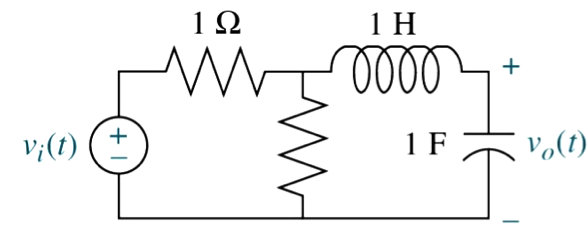
\includegraphics[width=0.5\textwidth]{testfig}
		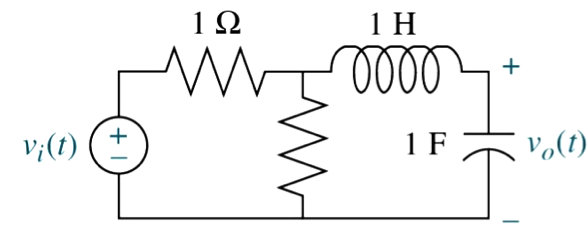
\includegraphics{testfig}
		\caption{\rajah}
		\label{fig:meshcircuit}
	\end{figure}

	% Table generated by Excel2LaTeX from sheet 'Sheet1'
	\begin{table}[H]
		\centering
		\caption{\jadual}
		\begin{tabular}{cc}
			\toprule
			\multicolumn{1}{l}{\textbf{Frequency}} & \multicolumn{1}{l}{\textbf{Impedance (Magnitude) ($\Omega$)}} \\
			\midrule
			5 Hz  & 20,000 \\
			10 Hz & 19,998 \\
			\vdots     & \vdots \\
			40 kHz & 602 \\
			50 kHz & 600 \\
			100 kHz & 600 \\
			\bottomrule
		\end{tabular}%
		\label{table:freqmag}%
	\end{table}%
\listclose % close 1st level question


% Question 2
\question

% question without enumerate list
Silver/silver chloride (Ag/AgCl) electrodes are commonly used in biological measurement.

\translation{Elektrod Argentum/Argentum chloride (Ag/AgCl) digunakan secara meluas didalam pengukuran biologi}	

\qmarks{5}

\listbegin	% start 1st level question
	\item \label{halfmembrane} State the definition of half-membrane
	
	\translation{Nyatakan definisi separuh-membran}
	
	\qmarks{2}
	
	\item \label{itm:net} Elaborate the basic mechanisms that contribute to condition in \ref{halfmembrane}, and write its net potential. % use label to reference to the list item
	
	\translation{Kembangkan mekanisma asas yang menyumbang kepada keadaan di \ref{halfmembrane}, dan tuliskan upaya bersih.}
	
	\qmarks{4}

	\listbegin % start 2nd level question
		\item \label{itm:ref2nd} Second level item that refer to \ref{itm:net}. Second level item. second level item. 
		
		\translation{ini adalah level kedua. ini adalah level kedua. ini adalah level kedua.} 
		
		\item Another second level that refer to \ref{itm:ref2nd}. Another second level. Another second level.
		
		\translation{ini adalah level kedua. ini adalah level kedua. ini adalah level kedua.} 
		
		\item Another second level that refer to \ref{itm:ref2nd}. Another second level. Another second level.
		
		\translation{ini adalah level kedua. ini adalah level kedua. ini adalah level kedua.} 
		
		\item Another second level that refer to \ref{itm:ref2nd}. Another second level. Another second level.
		
		\translation{ini adalah level kedua. ini adalah level kedua. ini adalah level kedua.} 


		\listbegin % start 3rd level question
			\item Another level. This is third level. This is third level. This is third level. This is third level
			
			\translation{Ini adalah level ketiga. Ini adalah level ketiga. Ini adalah level ketiga. Ini adalah level ketiga. Ini adalah level ketiga. Ini adalah level ketiga}

			\listbegin  % start 4th level question
				\item Another level. This is fourth level. This is fourth level. This is fourth level. This is fourth level. 
				
				\translation{Ini adalah level keempat. Ini adalah level keempat. Ini adalah level keempat. Ini adalah level keempat.}
			\listclose % close 4th level question
		\listclose % close 3rd level question
	\listclose % close 2nd level question
\listclose	% close 1st level question

% PART B
\newparten{Answer any THREE (3) questions} 

\newpartbm{Jawab mana-mana TIGA (3) soalan}
\bigskip

% Question 3
\clearpage	% start new page
\question

Some questions here...



\paperend
\end{lstlisting}

Additional command below generate:

\begin{lstlisting}[basicstyle=\footnotesize, frame=single]
% PART B
\newparten{Answer any THREE (3) questions} 

\newpartbm{Jawab mana-mana TIGA (3) soalan}

\bigkip 
% Question 3
\clearpage	% start new page
\question

Some questions here...


\end{lstlisting}

\begin{framed}
% PART B
\newpartenx{Answer any THREE (3) questions} 

\newpartbm{Jawab mana-mana TIGA (3) soalan}
\bigskip

\question{}

\end{framed}

\clearpage

The complete code to generate an exam paper using the method separating the question from the \verb|main.tex| is shown. 

\begin{lstlisting}[basicstyle=\footnotesize, frame=single]
\documentclass[12pt]{article}
\usepackage{finalxm}

%%%%%%%%%%%%%%%%%%%%%%%%
%%% SETUP TITLE PAGE %%%
%%%%%%%%%%%%%%%%%%%%%%%%
\mtefe{Akhir} 			% Akhir, Pertengahan
\semester{Kedua}		% Pertama, Kedua
\sidang{2017/2018}		
\examMonthYear{Jun 2018}
\courseCode{ENT390}
\courseNameEn{Bioinstrumentation 1}
\courseNameBM{Bioinstrumentasi 1}
\pagesbm{TIGA PULUH SATU}	% used if the number of pages exceeds 30
\durationhr{1 Jam}		% duration of exam
\makeatletter 
\if@minutes
\durationmin{30 Minit}	% MUST be enabled using \usepackage[minutes]{finalxm}
\fi 		
\makeatother	

\begin{document}
% cover page
\makecover

\instructionen{
This question paper has \textbf{TWO (2)} parts. Answer \textbf{all} questions in \mbox{\textbf{Part A}} and \mbox{\textbf{THREE (3)}} question in \mbox{\textbf{Part B}}. Each question contributes 25 marks.%
}
\instructionbm{%
Kertas soalan ini mengandungi \textbf{DUA (2)} bahagian. Jawab \textbf{semua} soalan di \mbox{\textbf{Bahagian A}} dan \mbox{\textbf{TIGA (3)}} soalan di \mbox{\textbf{Bahagian B}}. Setiap soalan menyumbang 25 markah.%
}

\makecoverend
% end cover page

%%%%%%%%%%%%%%%%%%%%%%%%%%%%
%%% MAIN BODY START HERE %%%
%%%%%%%%%%%%%%%%%%%%%%%%%%%%
\setmainstyle

% PART A
\newpartenx{Answer all questions} 

\newpartbm{Jawab semua soalan}
\bigskip

% Question 1
\question

\listbeginx	% start 1st level question
	\item \label{chemical} What chemical reactions you expect to see at these electrodes? 
	
	\translation{Apakah tindak balas kimia yang anda jangka dapat dilihat pada kedua –dua elektrod} 
	
	\qmarks{4}	% define marks
	
	\item A pair of biopotential electrodes is implanted in an animal to measure the electrocardiogram.
	
	\translation{Sepasang elektrod biopotensi diimplan ke dalam haiwan untuk mengukur elektrokardiogram.}

	\listbegin	% start 2nd level question
		\item Based on \ref{chemical}, explain what will happen if the electrodes were shorted together. Explain what will happen if the electrodes were shorted together. 
		
		\translation{Terangkan apakah yang akan berlaku apabila kedua – kedua elektrod disambung?. Terangkan apakah yang akan berlaku apabila kedua – kedua elektrod disambung?} 
		
		\qmarks{2} % define marks
	\listclose % close 2nd level question
	
	\item Explain what will happen if the capacitor in \cref{fig:meshcircuit} were shorted. 
	
	\translation{Terangkan apakah yang akan berlaku apabila kedua – kedua elektrod disambung?} 
	
	\qmarks{3} % define marks
		
	\begin{figure}[H] % H means, to put figure here after the code
		\centering
%		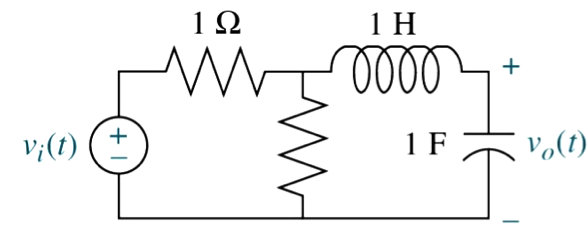
\includegraphics[width=0.5\textwidth]{testfig}
		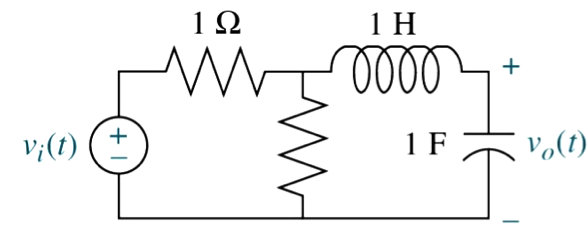
\includegraphics{testfig}
		\caption{\rajah}
		\label{fig:meshcircuit}
	\end{figure}

	% Table generated by Excel2LaTeX from sheet 'Sheet1'
	\begin{table}[H]
		\centering
		\caption{\jadual}
		\begin{tabular}{cc}
			\toprule
			\multicolumn{1}{l}{\textbf{Frequency}} & \multicolumn{1}{l}{\textbf{Impedance (Magnitude) ($\Omega$)}} \\
			\midrule
			5 Hz  & 20,000 \\
			10 Hz & 19,998 \\
			\vdots     & \vdots \\
			40 kHz & 602 \\
			50 kHz & 600 \\
			100 kHz & 600 \\
			\bottomrule
		\end{tabular}%
		\label{table:freqmag}%
	\end{table}%
\listclose % close 1st level question



% PART B
\newpartenx{Answer any THREE (3) questions} 

\newpartbm{Jawab mana-mana TIGA (3) soalan}
\bigskip

% Question 2
\question

% question without enumerate list
Silver/silver chloride (Ag/AgCl) electrodes are commonly used in biological measurement.

\translation{Elektrod Argentum/Argentum chloride (Ag/AgCl) digunakan secara meluas didalam pengukuran biologi}	

\qmarks{5}

\listbegin	% start 1st level question
	\item \label{halfmembrane} State the definition of half-membrane
	
	\translation{Nyatakan definisi separuh-membran}
	
	\qmarks{2}
	
	\item \label{itm:net} Elaborate the basic mechanisms that contribute to condition in \ref{halfmembrane}, and write its net potential. % use label to reference to the list item
	
	\translation{Kembangkan mekanisma asas yang menyumbang kepada keadaan di \ref{halfmembrane}, dan tuliskan upaya bersih.}
	
	\qmarks{4}

	\listbegin % start 2nd level question
		\item \label{itm:ref2nd} Second level item that refer to \ref{itm:net}. Second level item. second level item. 
		
		\translation{ini adalah level kedua. ini adalah level kedua. ini adalah level kedua.} 
		
		\item Another second level that refer to \ref{itm:ref2nd}. Another second level. Another second level.
		
		\translation{ini adalah level kedua. ini adalah level kedua. ini adalah level kedua.} 
		
		\item Another second level that refer to \ref{itm:ref2nd}. Another second level. Another second level.
		
		\translation{ini adalah level kedua. ini adalah level kedua. ini adalah level kedua.} 
		
		\item Another second level that refer to \ref{itm:ref2nd}. Another second level. Another second level.
		
		\translation{ini adalah level kedua. ini adalah level kedua. ini adalah level kedua.} 


		\listbegin % start 3rd level question
			\item Another level. This is third level. This is third level. This is third level. This is third level
			
			\translation{Ini adalah level ketiga. Ini adalah level ketiga. Ini adalah level ketiga. Ini adalah level ketiga. Ini adalah level ketiga. Ini adalah level ketiga}

			\listbegin  % start 4th level question
				\item Another level. This is fourth level. This is fourth level. This is fourth level. This is fourth level. 
				
				\translation{Ini adalah level keempat. Ini adalah level keempat. Ini adalah level keempat. Ini adalah level keempat.}
			\listclose % close 4th level question
		\listclose % close 3rd level question
	\listclose % close 2nd level question
\listclose	% close 1st level question
% Question 3
\clearpage	% start new page
\question

Some questions here...


% Question 4
\clearpage	% start new page
\question

Silver/silver chloride (Ag/AgCl) electrodes are commonly used in biological measurement. 

\translation{Elektrod Argentum/Argentum chloride (Ag/AgCl) digunakan secara meluas didalam pengukuran biologi}	

\listbegin	% start 1st level question
	\item \label{halfmembrane} State the definition of half-membrane
	
	\translation{some translation here}
	
	\qmarks{2}
	
	\answer{Put answer to this question here. This answer scheme can be turned on and off by executing \texttt{answers} option. Refer to manual for explanation.
	} 
	
	\item \label{itm:net} Elaborate the basic mechanisms that contribute to condition in \ref{halfmembrane}, and write its net potential. % use label to reference to the list item
	
	\translation{some translation here}
	
	\qmarks{2}
	
	\answer{Put answer to this question here. This answer scheme can be turned on and off by executing \texttt{answers} option. Refer to manual for explanation.
	} 

	\listbegin % start 2nd level question
		\item \label{itm:ref2nd} Second level item that refer to \ref{itm:net}. Second level item. second level item. \\
		\translation{ini adalah level kedua. ini adalah level kedua. ini adalah level kedua.} 
		
		\qmarks{3}
		
		\answer{Put answer to this question here. This answer scheme can be turned on and off by executing \texttt{answers} option. Refer to manual for explanation.
		} 

		\listbegin % start 3rd level question
			\item Another level. This is third level. This is third level. This is third level. This is third level\\
			\translation{Ini adalah level ketiga. Ini adalah level ketiga. Ini adalah level ketiga. Ini adalah level ketiga. Ini adalah level ketiga. Ini adalah level ketiga.}
		\listclose % close 3rd level question
	\listclose	% close 2nd level question	
\listclose	% close 1st level question	

% Question 5
\clearpage	% start new page
\question

	\answer{ 
		This is the answer to the question 5. This answer scheme can be turned on and off by executing \texttt{answers} option. Refer to manual for explanation.
	}




\paperend

\end{document}
\end{lstlisting}


\bigskip
In the \verb|question1.tex|, put you question for example,

\begin{lstlisting}[basicstyle=\footnotesize, frame=single]
\partQuestion
%\question{}

Silver/silver chloride (Ag/AgCl) electrodes are commonly used in biological measurement.

\translation{Elektrod Argentum/Argentum chloride (Ag/AgCl) digunakan secara meluas didalam pengukuran biologi}	

\qmarks{5}

\listbeginx	% start 1st level question
	\item \label{halfmembrane} State the definition of half-membrane
	
	\translation{Nyatakan definisi separuh-membran}
	
	\qmarks{2}

	\item \label{itm:net} Elaborate the basic mechanisms that contribute to condition in \ref{halfmembrane}, and write its net potential. % use label to reference to the list item

	\translation{Kembangkan mekanisma asas yang menyumbang kepada keadaan di \ref{halfmembrane}, dan tuliskan upaya bersih.}
	
	\qmarks{4}

	\listbeginx % start 2nd level question
		\item \label{itm:ref2nd} Second level item that refer to \ref{itm:net}. Second level item. second level item. 
		
		\translation{ini adalah level kedua. ini adalah level kedua. ini adalah level kedua.} 
		
	\listclose % close 2nd level question
\listclose	% close 1st level question
\end{lstlisting}
\clearpage

\section{Answer Scheme} \label{answerscheme}
You can also put your answer script here using \verb|answer| command. Note that the answers will only be visible when \verb|answers| option is called (refer to section \ref{package} in page~\pageref{package}).  

\begin{lstlisting}[basicstyle=\footnotesize, frame=single]
\question{}

Silver/silver chloride (Ag/AgCl) electrodes are commonly used in biological measurement.

\translation{Elektrod Argentum/Argentum chloride (Ag/AgCl) digunakan secara meluas didalam pengukuran biologi}\\	
\listbegin	% start 1st level question
	\item \label{halfmembrane} State the definition of half-membrane
	
	\translation{some translation here}
	
	\qmarks{2}
	
	\answer{Put answer to this question here
	} 
	
	\item \label{itm:net} Elaborate the basic mechanisms that contribute to condition in \ref{halfmembrane}, and write its net potential. % use label to reference to the list item
	
	\translation{some translation here}
	
	\qmarks{2}
	
	\answer{Put answer to this question here
	} 
	
	\listbegin % start 2nd level question
		\item \label{itm:ref2nd} Second level item that refer to \ref{itm:net}. Second level item. second level item. 
		
		\translation{ini adalah level kedua. ini adalah level kedua. ini adalah level kedua.} 
		
		\qmarks{3}
		
		\answer{Put answer to this question here}\\ 		
		\listbegin % start 3rd level question
			\item Another level. This is third level. This is third level. This is third level. This is third level.\\			
			\translation{Ini adalah level ketiga. Ini adalah level ketiga. Ini adalah level ketiga. Ini adalah level ketiga. Ini adalah level ketiga. Ini adalah level ketiga.}
		\listclose % close 3rd level question
	\listclose	% close 2nd level question	
\listclose	% close 1st level question	
\clearpage
\end{lstlisting}

\clearpage
\question{}

Silver/silver chloride (Ag/AgCl) electrodes are commonly used in biological measurement.

\translation{Elektrod Argentum/Argentum chloride (Ag/AgCl) digunakan secara meluas didalam pengukuran biologi}	

\listbegin	% start 1st level question
\item \label{halfmembranes} State the definition of half-membrane

\translation{some translation here}

\qmarks{2}

\answer{Put answer to this question here
} 

\item \label{itm:nets} Elaborate the basic mechanisms that contribute to condition in \ref{halfmembranes}, and write its net potential. % use label to reference to the list item

\translation{some translation here}

\qmarks{2}

\answer{Put answer to this question here
} 

\listbegin % start 2nd level question
\item \label{itm:ref2nds} Second level item that refer to \ref{itm:nets}. Second level item. second level item. 

\translation{ini adalah level kedua. ini adalah level kedua. ini adalah level kedua.} 

\qmarks{3}

\answer{Put answer to this question here
} 

\listbegin % start 3rd level question
\item Another level. This is third level. This is third level. This is third level. This is third level.

\translation{Ini adalah level ketiga. Ini adalah level ketiga. Ini adalah level ketiga. Ini adalah level ketiga. Ini adalah level ketiga. Ini adalah level ketiga.}
\listclose % close 3rd level question
\listclose	% close 2nd level question	
\listclose	% close 1st level question	

\clearpage

%\section{Figure}
%	\begin{figure}[H] % H means, to put figure here after the code
%		\centering
%		%		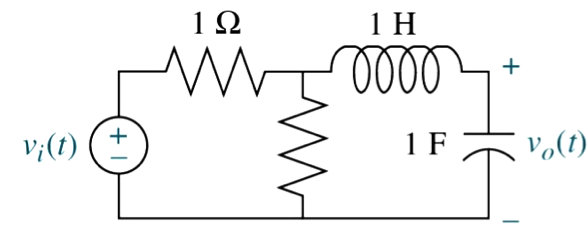
\includegraphics[width=0.5\textwidth]{testfig}
%		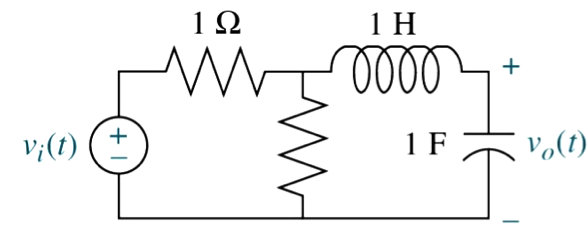
\includegraphics[scale=0.8]{testfig}
%		\caption{\translation{\bfseries Gambarajah~\thefigure}}
%		\label{fig:circuit}
%	\end{figure}
%
%\clearpage

\section{Landscape on Specific Page}
%https://tex.stackexchange.com/questions/9071/how-to-translate-and-rotate-the-heading-of-landscaped-pages
\verb|pdflscape.sty| can make the pdf page on landscape orientation. However, this package and other package such as \verb|typearea|, can't rotate the header and footer correctly. As a workaround, we need to disable the header and footer. This is the best solution for the time being. 

\begin{lstlisting}[basicstyle=\footnotesize, frame=single]
\newgeometry{top=2.54cm, bottom=-2.5cm, left=1cm, right=2.54cm}
\begin{landscape}
	\thispagestyle{empty}
	\begin{figure} % H means, to put figure here after the code
		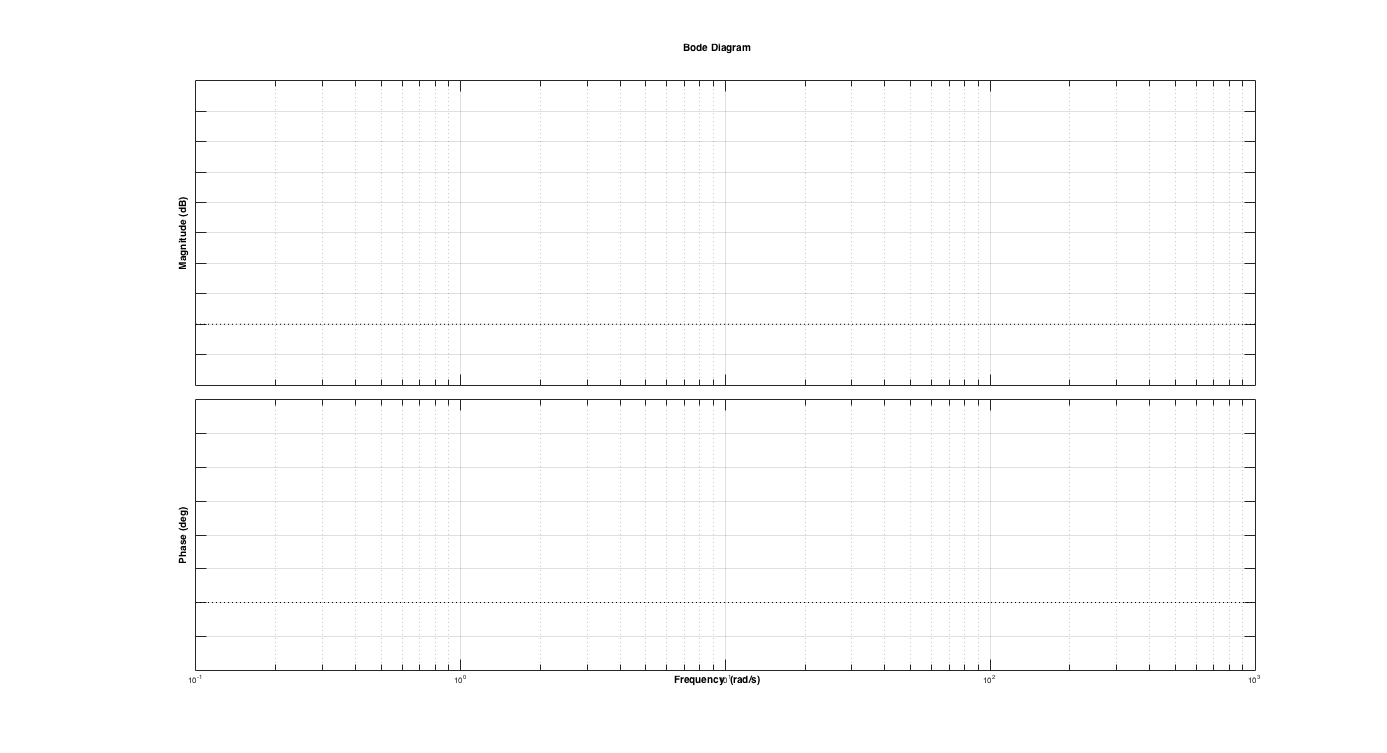
\includegraphics[scale=0.68]{bodeplot_appendix}
		\label{fig:bode}
	\end{figure}
\end{landscape}
\restoregeometry 
\end{lstlisting}

\newgeometry{top=2.54cm, bottom=-2.5cm, left=1cm, right=2.54cm}
\begin{landscape}
	\thispagestyle{empty}
	\begin{figure} % H means, to put figure here after the code
		%		\centering
		%		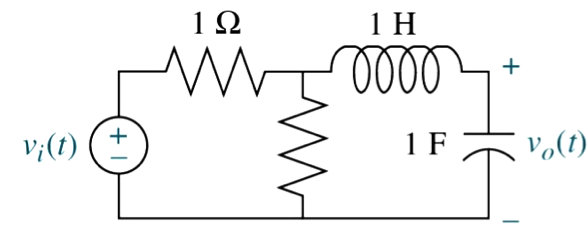
\includegraphics[width=0.5\textwidth]{testfig}
		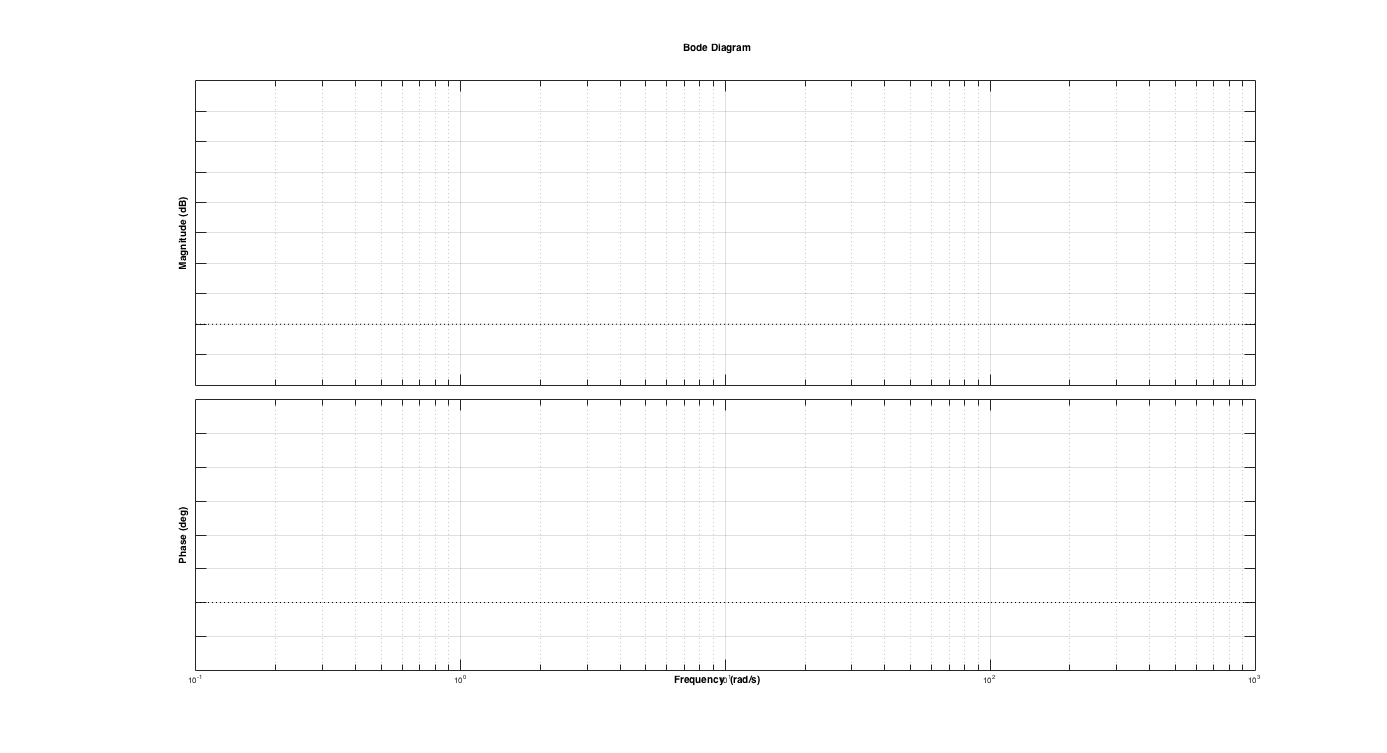
\includegraphics[scale=0.68]{bodeplot_appendix}
		%		\caption{\translation{\bfseries Gambarajah~\thefigure}}
		\label{fig:bode}
	\end{figure}
\end{landscape}
\restoregeometry 

\end{document}